\documentclass[conference]{IEEEtran}
\IEEEoverridecommandlockouts
% The preceding line is only needed to identify funding in the first footnote. If that is unneeded, please comment it out.
\usepackage{cite}
\usepackage{amsmath,amssymb,amsfonts}
\usepackage{graphicx}
\usepackage{textcomp}
\usepackage{xcolor}
\usepackage{hyperref}
\usepackage[utf8]{inputenc}
\def\BibTeX{{\rm B\kern-.05em{\sc i\kern-.025em b}\kern-.08em
    T\kern-.1667em\lower.7ex\hbox{E}\kern-.125emX}}
\begin{document}

\title{Replicação de servidores Memcached com Repcached\\
{\footnotesize Arquitetura master/slave em servidores memcached com libevent}
}


\author{\IEEEauthorblockN{Fabiano Araujo}
\IEEEauthorblockA{\textit{Universidade La Salle} \\
\textit{UNILASALLE}\\
Canoas, Brasil \\}
}

\maketitle

\begin{abstract}
Este artigo apresenta a utilização de Repcached como solução para replicação de Memcached, aproximando a solução de um ambiente tolerante a falhas por replicação.
\end{abstract}

\begin{IEEEkeywords}
cache, replication, memcached, repcached, distributed systems
\end{IEEEkeywords}

\section{Introdução}

Um sistema tolerante a falhas tem a capacidade de fornecer alta disponibilidade com consistência para seu uso em situações onde parte de sua funcionalidade ou de seus componentes para funcionar corretamente está defeituosa ou em falha total, de modo que o reparo possa ser realizado durante a falha sem a interrupção total ou parcial do sistema. \cite{Tanenbaum:2006:DSP:1202502}

O maior exemplo onde sistemas tolerante a falhas são necessários para prevenir problemas e acidentes são os aviões. Neles, a comunicação entre cada componente é crucial porém resistente a falhas onde é possível que um componente assuma a funcionalidade do outro em caso de falha completa ou perda do mesmo. Em alguns fabricantes é possível se ter quatro conjuntos de três processadores trabalhando paralelamente com o sistema de voto para que os comandos de navegação, conhecidos como \textit{fly-by-wire} cheguem ao seu resultado ideal. \cite{herman}

Em sistemas distribuídos a tolerância a falhas pode ser relacionada à transações bancárias, da necessidade de atomicidade, até a replicação de servidores de cache, da necessidade de disponibilidade. 

Servidores de cache são utilizados por diversos sistemas distribuídos que consumimos diariamente, inclusive em sistemas voltados para o entretenimento, como o Netflix, e sua principal finalidade é armazenar dados que não precisam ser atualizados constantemente e tornar-los disponível para acesso com uma grande velocidade de leitura, reduzindo custos de operação mecânica em discos ou tempo de execução de comandos.

Neste estudo é demonstrada a replicação, uma das técnicas de tolerância a falhas, em servidores Memcached \cite{memcached}, comumente utilizados por sistemas distribuídos, como Facebook ou Redit. Utilizando Docker \cite{docker}, os resultados obtidos são referentes ao experimento de parada e reinicialização de um elemento com defeito, neste caso um servidor de cache e o comportamento da aplicação o qual realiza a leitura dos dados periodicamente.

\section{Referencial Teórico}

Para o melhor entendimento do estudo, a compreensão básica dos princípios de tolerância a falhas é parte fundamental da compreensão da motivação da técnica de replicação. Junto dos conceitos simples, a compreensão da utilização de servidores cache e a arquitetura \textit{master/slave} também é fundamental para o entendimento completo de como os dados transitam entre os servidores e a razão pela qual a leitura é realizada, em geral, apenas em um tipo de servidor

\subsection{Tolerância a falhas}

Os principais componentes para a criação de um sistema tolerante a falhas podem ser resumidos em quatro tópicos diferentes: Disponibilidade, confiança, segurança e mantenabilidade \cite{Tanenbaum:2006:DSP:1202502}.

Disponibilidade é um dos principais conceitos a qual sistemas distribuídos podem ser exigidos principalmente em estruturas \textit{microservices}, cujo, assimilando com o anteriormente demonstrado modelo de aviação aonde os componentes são disjuntos e podem funcionar independentes, o sistema maior é dividido em pequenos módulos e estes módulos possuem um ecossistema específico para cada um deles, onde a falha de um não impacta de forma imediata o sistema como um todo. 

Assim a disponibilidade é um dos principais fatores a serem analisados neste estudo, visto que trata-se de servidores cache o qual a informação encontra-se para leitura especificamente neles. A discussão sobre a migração de sistemas de dados entre RDBMS (\textit{Relational Database Management System}) e NoSQL (\textit{Not-only SQL}), não é o objetivo deste artigo.

Confiança, por vezes confundida com disponibilidade, refere-se à propriedade que um sistema tem para rodar continuamente sem uma falha \cite{Tanenbaum:2006:DSP:1202502}. Difere-se da disponibilidade no ponto em que a disponibilidade é o mero fato de que o sistema está acessível e a confiança é a relação de frequência de erros sobre o tempo que impactam o acesso ao sistema. Por exemplo, se um \textit{host} desliga por um milissegundo a cada hora, pode-se dizer que o mesmo tem uma disponibilidade alta mas uma confiança pequena. Por outro lado, se um sistema para por duas semanas em um mês determinado do ano, pode-se dizer que o mesmo tem uma disponibilidade um pouco abaixo dos 100\%, porém a confiança é alta.

Quanto a segurança, é tendencioso pensar apenas no fato da segurança invasiva dos dados. No entanto, quando se tratando de tolerância a falhas, a segurança é a certeza de que quando um sistema se encontra em falha crítica nada catastrófico irá acontecer \cite{Tanenbaum:2006:DSP:1202502}. Citando a aviação, devido ao modelo adotado deste o lançamento das missões Apollo da NASA, a forma com que os dados são processados e outros componentes que possam assumir o mesmo papel em caso de falha, garantem que a aviação seja um dos sistemas mais seguros de transporte. \cite{herman}

Por fim, a mantenabilidade se refere a agilidade de reparo de um componente ou sistema em caso de falha. Com as recentes evoluções na área de inteligência artificial, é possível visualizar a utilização de \textit{deep learning} para eventuais correções sem que sejam necessárias intervenções humanas nestes sistemas.

É possível ainda definir os níveis de falha nos chamados modelos de falhas que se dividem em \textit{crash failure}, \textit{omission failure}, \textit{timing failure}, \textit{response failure} e \textit{arbitrary failure}.

Dentre todos, o mais arriscado, difícil de se diagnosticar sem verificação ativa de desenvolvedores é o \textit{arbitrary failure}, isto porque se caracteriza a falha aonde o dispositivo está enviando valores incorretos, porém todo seu funcionamento está correto. Normalmente se identificam por falhas de regras de negócios ou de erros de desenvolvimento.

A utilização de replicações de servidores cache tem como objetivo diminuir a ocorrência dos \textit{crash failures}, quando a aplicação ou servidor trava ou para de responder. 

\subsection{Servidores cache}

Servidores cache podem ser utilizados com diversos tipos de dados, mas seu principal objetivo é ser um servidor específico com dados que frequentemente são acessados e que não possuem armazenamento permanente. Dentre os tipos de servidores cache dois se destacam pela facilidade de utilização, o Redis e Memcached \cite{memcached}.

Estes são apenas exemplos de softwares de cache, onde nada impede que o carregamento de informações em espaço de memória possa ser implementado em demanda específica, sendo também uma forma de cache.

Fundamentalmente, no entanto, Redis não necessariamente é um servidor cache. Originado depois do Memcached, o Redis possui as características de um banco não relacional com as possibilidades de armazenamento de dados em RAM, o que permite uma leitura muito mais rápida e resposta para a solicitação em tempo incomparável com RDBMS normais. Sua principal diferença ao Memcached é a possibilidade de persistir os dados de forma nativa.

O Memcached por sua vez não possui funcionalidade de tipificação de dados armazenados ou mesmo a persistência em disco físico, todos os dados ficam armazenados em RAM e, por isto, possui uma necessidade maior em relação aos cuidados de tolerância a falhas, visto que uma vez o software ou dispositivo serem desligados, as informações são perdidas e novo reabastecimento dos dados deve ser realizado.

Em ambos os softwares, os valores são armazenados na estrutura chave-valor, onde o Redis armazena o tipo de informação junto dos dados permitindo operações complexas de ordenação ou estrutura de filas simplesmente encadeadas, do contrário do Memcached que armazena a estrutura em valor \textit{string} apenas.

O Redis possui, nativamente, a possibilidade de distribuição de processamento em clusters e replicação de servidores com estrutura \textit{master/slave}. O Memcached por outro lado, não oferece nenhum dos dois. A solução mais próxima de replicação é a utilização de Repcached \cite{repcached}


O cache também é implementado em menores versões como nos navegadores atuais que possuem cache local de arquivos estáticos como JavaScripts, CSS e imagens. Além deste cache local, é possível também o controle de balanceamento de acesso de dados por outros servidores de cache interligados ou não, como demonstra a figura 1.

\begin{figure}[h!]
\centerline{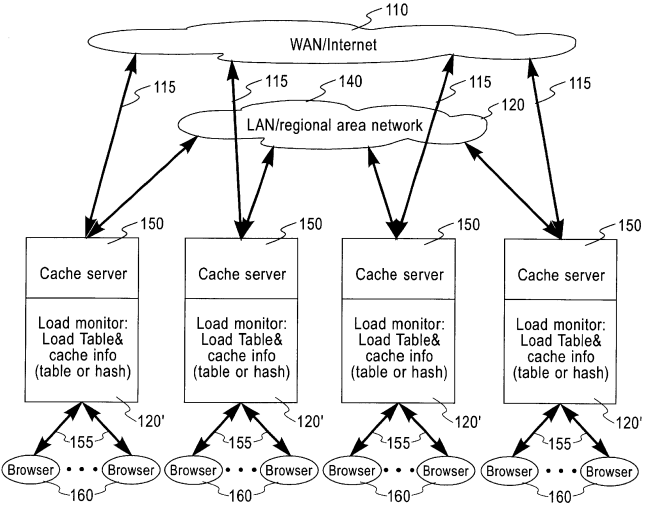
\includegraphics[width=0.7\linewidth]{figura1.png}}
\caption{Arquitetura de caches \cite{cachepatent}}
\label{fig}
\end{figure}

A figura 1 ainda demonstra fatores a serem abordados pela replicação de servidores e omite a estrutura \textit{master/slave} de alguns softwares. O exemplo da figura 1, no entanto, mostra a relação de conectividade padrão de algumas aplicações, como os navegadores. 

Visualizando a imagem como uma forma de fluxo para os servidores externos, onde este estariam disponíveis via WAN (servidor de base de dados, por exemplo) os servidores de caches estão dispostos com a finalidade de permitir acesso mais rápido às informações previamente carregadas e são conectados em uma rede LAN para comunicarem entre si.

\section{Implementação}

O experimento realizado para demonstração da ferramente se dispôs entre dois \textit{containers} Docker\cite{docker}, obtidos de uma imagem com todos as bibliotecas necessárias para execução de dois servidores Repcached \cite{repcached} isolados.

A replicação fica por parte da definição cíclica dos IPs de servidor \textit{master} e \textit{slave}. Por vezes a definição da dependência ficou confusa e foi obtido o entendimento de que o a definição real entre \textit{master} e \textit{slave}, nesta ocasião, refere-se especificamente à escolha do desenvolvedor ou cliente de utilização de um IP.

Utilizando imagens pré definidas dos \textit{containers}, algumas modificações foram realizadas para que pudesse ser exibida de forma coerente a comunicação entre os servidores nos \textit{containers}. Isto porque os exemplos encontrados e fundamentados nas próprias imagens utilizadas como exemplo utilizam do próprio \textit{host} de um \textit{container} Docker com o próprio \textit{container}, não deixando clara as limitações da comunicação entre dois \textit{containers}.

Da imagem \textit{yrobla/docker-repcached} \cite{yrobla}, foram retirados os arquivos que criavam a possibilidade de logins com administradores, por não ser relevante ao experimento e, principalmente, foi postergada a inicialização do \textit{daemon} Memcached. Mesmo que o projeto possua um nome diferente, Repcached, o mesmo é uma adaptação do Memcached adicionando apenas um parâmetro para identificação do IP do servidor cujo terá replicação dos dados.

A postergação da inicialização se fez necessária pelo contexto de utilizar dois \textit{containers} Dockers. Em sua natureza, cada \textit{container} possui um IP local cujo, por padrão, é definido por um dispositivo virtual de rede. Este dispositivo funciona como um DHCP entre \textit{containers} atribuindo os IPs assim que o \textit{container} for iniciado.

No código inicial no entanto era necessário definir o IP do servidor \textit{slave} antes da inicialização. Porém como a inicialização é o evento que é atribuído um IP na rede virtual interna de \textit{containers} Docker, não era possível definir a atribuição, gerando uma falha no procedimento pois o mesmo adotava o IP 127.0.0.1 caso não fosse especificado.

Exposta a porta 11211, padrão do servidor memcached, então, é inicializado o \textit{container} e acessado o mesmo utilizando as diretivas \textit{exec -it --entrypoint /bin/bash} para que se tenha acesso à um \textit{shell} onde é possível iniciar o servidor memcached. 

Iniciando os dois \textit{containers} foi então verificado os IPs internos definidos pelo comando \textit{docker network inspect bridge}. Tomando nota dos IPs atribuídos, os serviços memcached foram iniciados em ambos os \textit{containers} apontando o parâmetro \textit{-x} para o IP do \textit{container} oposto. Por isto a atribuição de \textit{master} e \textit{slave} se tornou cíclica.

Tal comportamento permite que caso o \textit{slave} caia e retorne em um momento posterior, o mesmo possua todos os dados de \textit{master} e vice-versa. Diferente de estruturas como Redis que possui \textit{slaves} como apenas leitura e propagação direta para \textit{master}. Da forma como o Repmemcached é organizado ambos possuem a mesma atribuição

Omitir a definição do IP ou tornar a atribuição do IP pelo parâmetro \textit{-x} para 127.0.0.1 inviabiliza o fluxo, sendo necessário reiniciar todo o processo em \textit{master} caso o \textit{slave} caia. 

A estrutura utilizada no experimento pode ser visualizada na figura 2.

\begin{figure}[h!]
\centerline{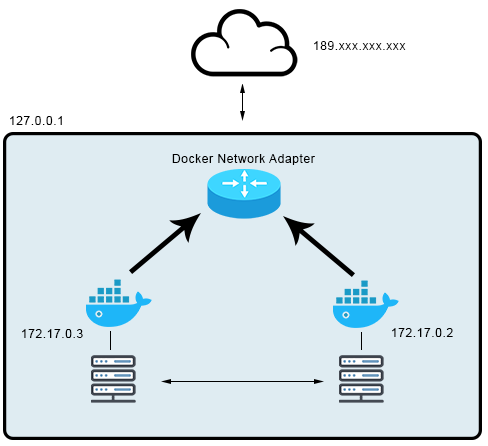
\includegraphics[width=1\linewidth]{figura2.png}}
\caption{Ambiente de experimento}
\label{fig}
\end{figure}

\section{Resultados} 

Foi possível realizar a replicação de ambientes Memcached com Repcached com sucesso entre \textit{containers} Docker. Uma vez iniciados os \textit{containers}, foi identificado os IPs dos mesmos e finalmente iniciados os serviços via \textit{nohup}, uma vez que os parâmetros estavam melhor dispostos se explicitamente inseridos

Foram nomeados cache1 e cache2 respectivamente e tratada a conectividade de uma aplicação PHP com o cache2, sendo este ponto de entrada de obtenção e escrita da aplicação. Em termos de utilização, pode-se afirmar que a aplicação interagiu diretamente apenas com o cache2 e que devida a funcionalidade de replicação, o cache1 foi alimentado de forma semelhante.

No momento do ensaio de uma queda, para que a aplicação pudesse continuar a consumir de um servidor Memcached, foram atribuídos dois IPs de servidores com pesos distintos. O peso do servidor, no contexto de aplicação PHP, segundo a sua documentação define a prioridade com que a conectividade irá acontecer, assim o servidor com peso maior terá prioridade e uma vez que não for possível conectar, tentara o segundo mais próximo \cite{phpmemcachedserver}. Não é definida a forma de utilização caso os servidores tiverem o mesmo peso.

Em código PHP, é possível definir servidores de replicação dos dados, porém nada condiz com a replicação de informação integral que o Repcached se propõe. Das diretivas do PHP, o que se tem de replicação é a replicação imediata da chave salva pelo próprio script PHP, porém chaves criadas por terceiros não serão replicadas visto que não comunicação entre os servidores.

A replicação em código PHP também não permite que os dados armazenados sejam recuperados em caso de queda de um dos servidores, assim servindo apenas para a replicação em servidores com finalidades distintas ou que possuam replicação não conjunta, isto é, entre outros dois servidores que não se comunicam diretamente.

A aplicação contou com um endpoint em AJAX que demonstrava a informação armazenada diretamente por \textit{telnet}, utilizando das diretivas, uma vez estabelecida conexão com Memcached de \textit{get} e \textit{set}.

Em outro experimento, foi realizada a conexão entre três Dockers, no intuito de aumenta a complexidade cíclica para três servidores. O experimento no entanto falhou pelo motivo de funcionalidade da biblioteca libevent. Dado o ambiente como demonstrado na figura 3, uma entrada no servidor \textit{slave 1} não estaria armazenado do \textit{slave 2}, mas apenas no \textit{master}, pois o \textit{slave 2} está tanto recebendo a informação como enviando para outro servidor que não se comunica diretamente com o ele, no caso, \textit{master}. 

Tal conclusão inviabiliza a utilização de Repmemcache em ambientes que demandam grande complexidade de tolerância a falhas ou que necessitem de um controle de alta disponibilidade visto que conforme seus autores, o Memcached não foi construído como um servidor de alta disponibilidade.

\begin{figure}[h!]
\centerline{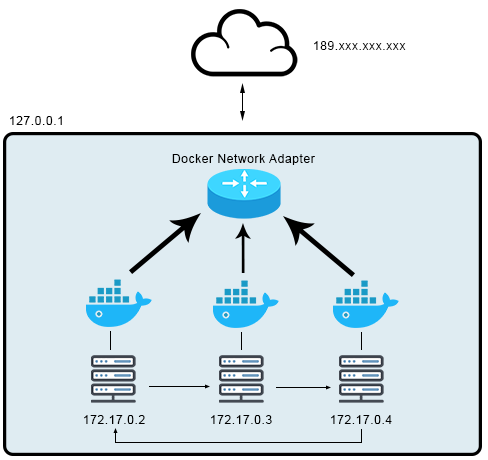
\includegraphics[width=1\linewidth]{figura3.png}}
\caption{Ambiente de experimento com três replicações}
\label{fig}
\end{figure}

\section{Conclusão}

Por meios padrão, não é possível obter a replicação do ambiente Memcached, visto que o mesmo não possui instruções nem foi moldado para tal. Sua natureza de armazenamento de dados apenas em RAM também não prevê qualquer persistência de dados físicos que pudessem justificar a adaptação de outro serviço como leitura dos seus dados.

Assim o uso do Repcached permite a criação de um servidor \textit{master} e um \textit{slave} diretamente conectados, mas não permite a criação de \textit{clusters} de informação. A replicação também não acontece em termos de processamento mas apenas de indicação de lugar na memória em outro endereço de rede além do servidor \textit{master}, não configurando assim o comportamento de \textit{cluster}.

A definição de que o Memcached não possui alta disponibilidade impacta diretamente no consumo atual da informação, dada a vasta capacidade tecnológica que outra ferramentas tem neste assunto, como Redis. Cabe aos desenvolvedores e analistas identificarem a utilização do Memcached detalhadamente para evitar perigos de inviabilidade de comunicação por parte de falta de replicação.

\bibliographystyle{IEEEtran}
\renewcommand{\refname}{Referências}
\bibliography{References}
\end{document}